\chapter{Исследование тематического профиля Интернет-СМИ Омской области} \label{chapt2}
\section{Цели и дизайн исследования}
В данной части работы мы разработаем и проведём исследование, \textbf{цель} которого состоит в построении тематического профиля Интернет-СМИ Омской области и, затем, определении в этих темах очагов социальной напряжённости. На примере данного исследования будут показаны возможности метода интеллектуального анализа текста в социологии и дано представление о том, как конкретно и с использованием каких инструментов пройти все ранее выделенные этапы интеллектуального анализа текста. Исследование тематического профиля будет включать в себя следующие \textbf{задачи}:

\begin{enumerate}
\item Оценка доступности и характера данных. Сбор данных.
\item Предварительная обработка данных.
\item Тематическое моделирование:
	\begin{enumerate}
	\item Определение оптимального количества тем.
	\item \textbf{Построение тематического профиля омских Интернет-СМИ.}
	\end{enumerate}
\item Анализ комментариев:
	\begin{enumerate}
	\item Составление рейтинга тем по их комментируемости.
	\item Создание тонального словаря.
	\item Составление рейтинга тем, по комментируемости.
	\item \textbf{Составление рейтинга тем по социальной напряжённости.} Индикатором социальной напряжённости выступает эмоциональная тональность комментариев к статьям данной тематики.
	\end{enumerate}

\end{enumerate}

Все задачи тесно связаны друг с другом. Корректное решение любой из представленных выше задач невозможно без решения предыдущих. Задача составления рейтинга тем по социальной напряжённости является, таким образом, кульминацией исследования, заключающим шагом в цепи задач. Именно в ней наиболее конкретно выражена цель исследования в этой части работы.

\section{Оценка доступности и характера данных. Сбор данных}
Прежде чем начать сбор данных, нам придётся поставить перед собой несколько вопросов, представляющих особенную трудность в исследованиях данного типа. А именно, необходимо определить, что будет являться носителем знаний по исследуемой проблеме (т. е. эмпирическим объектом исследования), каковы границы генеральной совокупности, какой метод будет являться адекватным для построения выборочной совокупности, как определить качественные и количественные характеристики выборки, каковы критерии репрезентативности выборки \cite{methodlogy_internet}.

\subsection{Определение эмпирического объекта} 

В исследованиях подобного вида эмпирическим объектом могут быть посты, комментарии, отдельные высказывания и многое другое. В нашем случае можно сказать, что источником знаний о проблемах, затронутых в данном исследовании являются новостные статьи в Интернет-СМИ Омской области. Углубляясь дальше, мы должны решить какие аспекты статей нас интересуют. Статья в Интернет-СМИ -- не просто текст. Это документ, который имеет свою структуру. В этой структуре нас буду интересовать такие элементы как собственно текст, название, дата публикации, комментарии к статье, принадлежность к тому или иному СМИ. Первая причина, по которой они были выбраны состоит в представленности этих элементов в статьях каждого из рассматриваемых нами Интернет-СМИ. Количество просмотров и ключевые слова (тэги), например, на некоторых ресурсах бывают не указаны. Другая причина -- достаточность данных элементов для решения исследовательских задач.

\subsection{Определение генеральной и выборочной совокупностей}

Определение эмпирического объекта позволяет перейти к установлению генеральной и выборочной совокупностей. На сегодняшний день не существует единой позиции как определять эти совокупности при исследовании текстов в сети Интернет. Каждый исследователь придумывает сам, каким способом наиболее полно реализовать принципы выборки.

Зизи Папачарисси \cite{zizi}, например, при исследовании блогосферы в качестве генеральной совокупности определяла все блоги, расположенные на платформе blogger.com. Она объясняет свой выбор тем, что это наиболее популярный и большой по числу блогеров англоязычный сайт, который предоставляет возможности для персональных публикаций в стиле любительской журналистики. Любой блог, по мнению Папачарисси, размещённый на этом сайте, представляет собой единицу анализа, отвечающую по своим характеристикам признакам принадлежности к генеральной совокупности. Однако нельзя согласиться, что блоги с blogger.com репрезентативны относительно всей блогосферы. Выборочную совокупность блогов Папачарисии составляла использую случайную отправную точку и случайный выборочный интервал. Однако исследователем не было оговорено, какие именно данные вводились в поисковую систему для поиска релевантных блогов и какие именно блоги считались релевантными, сколько блогов входило в генеральную совокупность и почему было отобрано именно 260. К тому же использование поисковых систем для поиска блогов выглядит сомнительно: алгоритмы данных систем неизвестны исследователю и нельзя сказать, почему были отобраны эти блоги, а не иные.

Генеральную совокупность в нашем исследовании составляют новостные статьи Интернет-СМИ г. Омска. Омским Интернет-СМИ считается веб-сайт, ставящий своей задачей выполнение функции средства массовой информации (СМИ) в сети Интернет и ориентированный на аудиторию, живущую в Омской области. По данным Агентства Региональных Исследований за июнь 2014 года в Омске работает около 18 Интернет-СМИ с месячным количеством уникальных посетителе в месяц более 10000 \cite{ari_rating}.

Использование данных со всех возможных ресурсов -- очень трудоёмкая задача, поскольку добавление нового источника требует практически полного переписывания соответствующей части компьютерной программы, ответственной за собственной сбор данных, и частичной переработки модуля предварительной обработки. Вполне привычным для социолога решением будет конструирование выборки. Однако, как рассчитать выборку, если не известны объёмы генеральной совокупности? А даже если бы мы знали количество статей каждого из рассматриваемых Интернет-СМИ за любой промежуток времени, разве было бы корректно использовать традиционные методы определения выборочной совокупности в такого типа исследованиях? Эта аналогия видится некорректной по причине кардинального различия эмпирических объектов -- человека и текста. При определении людей в качестве эмпирических объектов исследования социолог как правило предполагает, что они в равной степени могут служить источником информации о проблеме. Исключение из этого правила встречается, когда исследователь дополнительно изучает мнение экспертов. Но такие опросы -- это отдельная часть исследования, в которой как правило используются другие методы сбора и анализа информации.

Тексты в Интернете не равнозначны по своему значению. По нашему мнению, новостная статья заслуживает тем больше внимания, чем больше количество её просмотров. Статья, которую никто не прочитал, -- не существует в медийной сфере. %Но не все Интернет-СМИ предоставляют эту информацию, поэтому можно опереться на косвенный индикатор -- количество просмотров всех статей исследуемого ресурса. То есть мы предполагаем, что чем больше совокупное количество просмотров у одного ресурса, тем более сильно влияние каждой его отдельной статьи.

В нашем случае необходимо определить несколько Интернет-СМИ, все статьи которых будут отобраны для исследования. Мы решили, что при определении значимости статьи определяющей характеристикой является количество просмотров. Хотя Интернет-СМИ в Омске и немало, не все из них одинаково популярны. Судя по тем же данным АРИ \cite{ari_rating}, в Омске существует всего четыре новостных ресурса, страницы которых просматривают более одного миллиона раз в месяц. На их долю приходится 65\% всех просмотров. Представляется, что анализ статей, получивших более половины всех просмотров является достаточным основанием для выделения их в качестве выборочной совокупности, по результатам анализа которой можно будет делать выводы об омских Интернет-СМИ в целом. Таким образом в исследовании будут проанализированы все новостные статьи с сайтов <<Город 55>>\footnote{\href{http://gorod55.ru}{http://gorod55.ru}}, <<БК55>>\footnote{\href{http://bk55.ru}{http://bk55.ru}}, <<НГС Омск>>\footnote{\href{http://ngs55.ru}{http://ngs55.ru}}, <<Омск-Информ>>\footnote{\href{http://omskinform.ru}{http://omskinform.ru}} за период с 1 сентября 2013 по 1 сентября 2014. Новостными статьями будут считаться те, которые публикуются на данном ресурсе в разделе <<Новости>>. Статьи из категорий <<Работа>>, <<Объявления>>, <<Блоги>> и др. в анализе не участвуют.

Определившись с данными, которые необходимо собрать, нужно решить, каким способом это сделать, т. е. с использованием каких инструментов и технологий будет производится сбор данных. Для этого мы будем использовать язык программирования Python, который широко используется для анализа данных. Основанием для такого выбора является его простота, поддержка многопоточности, что полезно для более быстрого сбора данных, наличие сторонних библиотек, что позволяет избежать написание рутинного кода, а также то, что обработка и анализ данных также будет производится на этом языке -- это обеспечивает некоторую консистентность исследования. Ближайшей альтернативой данному решению нам видится использование программной платформы node.js из-за хорошей поддержки асинхронных запросов (и, следовательно, высокой скорости) и наличия множества качественных библиотек для сбора данных или языка R, который традиционно популярен в академической среде для сбора и анализа данных.

Для хранения данных использовалась база данных MongoDB. Как говорилось выше, в БД будут присутствовать следующие поля: называние статьи, содержимое статьи, ссылка на статью, дата публикации, количество комментариев и список комментариев к статье. Статьи с каждого источника сохранялись в отдельной коллекции.

\subsection{Результаты сбора данных}

Результаты сбора данных следующие представлены в диаграмме на рисунке \ref{fig:doc_number}
\begin{figure}[h!]
	\centering
	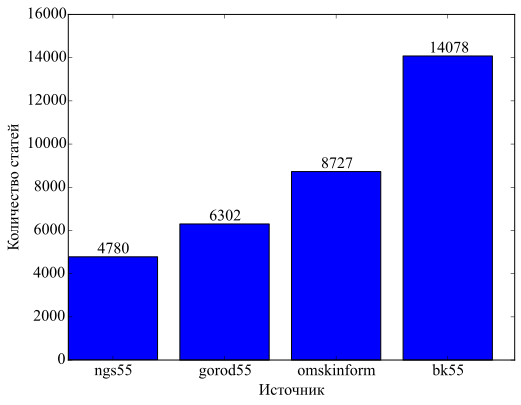
\includegraphics[totalheight=10cm]{doc_number}
	\caption{Количество статей по источникам}
	\label{fig:doc_number}
\end{figure}

\begin{comment}
\begin{itemize}
\item C сайта gorod55.ru было собрано 6302 статьи
\item Больше всего новостных статей за указанный промежуток времени было опубликовано на bk55.ru -- 14078 статей на bk55.ru
\item Наименьшее количество статей -- 4780 -- было найдено на ngs55.ru
\item 8727 статей по указанным параметрам было собрано с сайта omskinform.ru
\end{itemize}
\end{comment}


Всего, таким образом, в анализе участвовало 33887 статей.

На этом этапе крайне важно контролировать корректность и полноту собираемых данных. Сложнее всего было с сайтом bk55.ru, поскольку в нём использовались несколько различных шаблонов для отображения информации, каждый из которых необходимо было отследить и создать под него набор правил для извлечения данных.

\begin{figure}[h!]
	\centering
	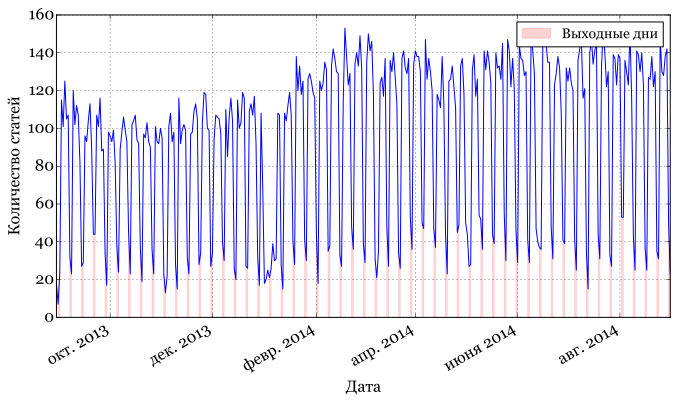
\includegraphics[totalheight=10cm]{docs_by_day}
	\caption{Количество статей по дням}
	\label{fig:docs_by_day}
\end{figure}

Исследуем распределение статей во времени, построив график (рисунок \ref{fig:docs_by_day}), на оси $x$ которого отложены дни, а на оси $y$ -- количество статей, опубликованных в каждый из дней. Дополнительно выделим область под графиком, соответствующую выходным дням красным цветом.

Анализ графика позволяет сделать несколько выводов. Во-первых, заметна неравномерность распределения статей по дням недели. В будние дни в среднем публикуется статей 116, в то время как в выходные -- только 33. Во-вторых, наблюдается сильное снижение количества публикаций на новогодние каникулы. Наблюдаемые колебания очевидно зависят от рабочего графика сотрудников СМИ.

\section{Предварительная обработка данных}

Предварительная обработка данных -- один из важнейших этапов в анализе текста. Наша цель на этом этапе -- удаление несущественных и вносящих помехи данных и преобразование данных к удобному для анализа виду.

На самом деле удалять несущественные данные мы начали ещё на этапе сбора данных, поскольку перед записью в базу данных весь текст, если это было необходимо, очищался от HTML-разметки. Преобразование же данных на том этапе заключалось в конвертации текста, содержащего информацию о дате публикации, в специальный тип данных, позволяющий обращаться к этим данным как к дате, например, производить выборку статей за определённый период.

Дальнейшая обработка данный заключалась в следующем:

\begin{enumerate}
\item Удаление лишней информации
\item Перевод текста в нижний регистр
\item Токенизация
\item Удаление пунктуации
\item Лемматизация
\item Удаление стоп-слов
%\item Замена слов
\end{enumerate}
Поясним некоторые из этих этапов.

\paragraph{Удаление специфических признаков.}
Данный этап предварительной обработки данных заключается в удалении из каждой статьи признаков, свидетельствующих о её принадлежности к какому-либо источнику. Если посмотреть на полученные тексты, то можно увидеть, что редакция каждого СМИ устанавливает собственные правила оформления документов, касающиеся оформления ссылок на источники данных, фотографий, указание имён авторов. В случаем если эти отличительные черты не будут устранены, алгоритмы тематического моделирования, которые мы в дальнейшем собираемся применить к собранному корпусу текстов, будут стремиться образовать темы вокруг источников. Процедура унификации статей из различных источников достаточно трудоёмка и требует ручного анализа множества статей с каждого из них, с тем чтобы выявить в них специфические черты для каждого сайта. Такими чертам могут быть имена журналистов данного издания или правила оформления фото и видео материалов (например, около каждой фотографии может указываться копирайт).

Например, чтобы удалить имена журналистов из текстов статей на сайте bk55.ru, необходимо было, во-первых, составить их список. Для составления списка, на языке python была написана программа, выводящая два последних слова каждого документа, если они начинались с заглавной буквы (как правило имена авторов указывались в конце документа, хоть и не всегда). Из полученного списка примерно в пятьсот пар были вручную отсеяны пары, не являющиеся именем и фамилией. Те пары из этого списка, которые встречались больше двух раз, считались нами именем и фамилией журналистов сайта bk55.ru. На последнем этапе фамилии журналистов удалялись из каждого документа. К тому же, так как после имён журналистов часто указывалась другая метаинформация (главным образом ссылки источники информации), то также удалялся весь текст после имён, если по размеру этот текст не превышал определённое количество символов (чтобы предотвратить удаление не метаинформации.

После устранения специфической информации данные из различных источников объединялись в единый корпус и подвергались дальнейшей обработке.

\paragraph{Токенизация.}
Следующим этапом предварительной обработки текста является токенизация. Именно с неё начинается обработка естественного языка как наука и как конкретная деятельность \cite{Webster1992}. Под токенизацией понимают процесс сегментации текста на отдельные части, называемые токенами. Именно токены являются теми первичными элементами, которые непосредственно участвуют в процессе анализа. 

Выделяют два основных признака токена -- лингвистическая значимость (Токен обладать смыслом, нести некоторое значение. Лингвистическая значимость токена <<мать-и-мачеха>> полнее, чем значимость пяти отдельных токенов <<и>>, <<->>, <<->>, <<мачеха>> и <<мать>>) и методологическая полезность (формулировка токена должна помогать достижению цели исследования) \cite[стр. 1106]{Webster1992}. В языках с иероглифической письменностью токенизация является серьёзной проблемой, поскольку один иероглиф может обозначать как морфемы (в таком случае он не удовлетворяет требованиям для того, чтобы считаться токеном), так и целые слова. В английском и русском языках проблема токенизации не стоит так остро и чаще всего токены определяются через пробелы между словами и знаки препинания. Тем не менее, даже в этих языках существуют определённые нюансы.

Нами было протестировано несколько алгоритмов токенизации (токенайзеры TreebankWordTokenizer, WordPunctTokenizer, PunctWordTokenizer и WhitespaceTokenizer из программы NLTK\footnote{\href{http://www.nltk.org}{http://www.nltk.org}} и токенайзер из Pattern\footnote{\href{http://www.clips.ua.ac.be/pattern}{http://www.clips.ua.ac.be/pattern}}). Корректнее всех выделял токены изначально не предназначенный для работы с русским языком токенайзер из программы Pattern. Например, он единственный интерпретировал URL'ы как цельные токены, не выделяя в них отдельные сегменты на основе знаков препинания (<<http://www.omsu.ru/>>, а не, например, <<http>>, <<://>>, <<www>>, <<.>>, <<omsu>>, <<.>>, <<ru>>, <</>>).

\paragraph{Стемминг и лемматизация.}
После токенизации и удаления токенов, являющихся знаками препинания, мы перешли от представления документов как набора символов к документам как списку слов. Дальнейшие наши шаги будут направлены на уменьшение длинны этого списка, т. е. на снижение как общего количества токенов, так и количества их уникальных единиц. Необходимость этих шагов обусловлена желанием снизить вычислительную сложность анализа данных.

Первый шаг направлен на снижение количества уникальных токенов. Для компьютера различные формы одного и того же слова являются совершенно разными словами. Существует два способа для приведения словоформ к одной лексеме. Первый, самый простой, называется стемминг. Он состоит в отсечении слово- и формообразующих частей -- префиксов, суффиксов, окончаний, в результате чего остаётся основа слова -- неизменная часть, выражающая его лексическое значение.

Более сложным подходом к решению проблемы унификации словоформ является лемматизация. Лемматизация -- это процесс приведения словоформы к лемме — её нормальной (словарной) форме. В русском языке нормальная форма имени существительного имеет именительный падеж и единственной число, для прилагательных добавляется требование мужского рода, а глаголы, деепричастия и причастия в нормальной форме должны стоять в инфинитиве.

Для постановки слова в нормальную форму необходимо иметь словарь, где для каждого слова определены его характеристики, т. е. часть речи, падеж, число, род, форма глагола (если это глагол). Создание такого словаря требует колоссальных трудов. В отличии от этого, стемминг предполагает наличие лишь списка приставок, суффиксов и окончаний, количество которых исчисляется несколькими десятками. К счастью, для русского языка существует так необходимый для лемматизации словарь, созданный в рамках проекта OpenCorpora\footnote{\href{http://opencorpora.org}{http://opencorpora.org}}. Использующая этот словарь программа pymorphy2\footnote{\href{https://pymorphy2.readthedocs.org}{https://pymorphy2.readthedocs.org}} позволяет приводить слова к нормальной форме.

Между вышеозначенными способами мы выбрали лемматизацию, поскольку получаемые в результате этого процесса леммы удобнее интерпретировать, по сравнению с усечёнными основами слов, значение которых не всегда легко восстановить.

\paragraph{Удаление стоп-слов.}
Дальнейшие усилия по уменьшению количества токенов связаны с удалением так называемых стоп-слов. Эти слова, сами по себе почти не неся полезного смысла, тем не менее, необходимы для нормального восприятия текста. Чаще всего к разряду стоп-слов относятся служебные части речи -- предлоги, союзы, частицы. Будучи широко распространёнными в тексте, они мало могут сказать о его теме.

В качестве базы для списка стоп-слов был использован список русских стоп-слов из программы NLTK. Однако его нельзя считать достаточно полным. Включая в себя 151 слово, данный список покрывает лишь самые основные случаи. Для его пополнения необходимо обратиться к собранным ранее данным. На их основе мы составили список наиболее часто встречающихся в корпусе токенов. Среди них выбрали несколько десятков, наиболее точно подходящие под описание стоп-слов (это, который, такой, некоторый, другой, тот и др.), которые затем добавили в соответствующий список. Представляется, что такой список, дополненный словами, выбранными из числа наиболее распространённых, является достаточно полным, поскольку стоп-слова по своему характеру всегда относятся к наиболее часто встречающимся в тексте. Редкие слова, как правило, свидетельствуют о принадлежности текста к какой-либо теме, а потому не могут относиться к разряду стоп-слов.

%\subsubsection{Замена слов}
%В заключение, для удобства анализа была произведена замена некоторых слов. Данная замена включала в себя, во-первых, раскрытие аббревиатур (рф $\to$ россия, ул $\to$ улица и др.), а во-вторых, лемматизацию токенов, которые не были лемматизированы автоматически (расина $\to$ расин, парка $\to$ парк). Данный шаг не является обязательным и может быть без последствий пропущен.

\paragraph{Выводы.}
Как видно, в общих чертах данный набор процедур повторяет составляющие предварительной обработки данных из методологии CRISP-DM.

Необходимо отметить, что после каждой операции с данными на этапе предварительной обработки следует контролировать последствия производимых изменений. Такой контроль поможет выявить проблемы на раннем этапе, что убережёт от лишней работы в будущем\footnote{Например, одной из таких проблем, выявленных на раннем этапе, было наличие в текстах некоторых СМИ неразрывных пробелов. Они мешали токенизации, поскольку сегментация производилась по обычным пробелам. Так как визуально неразрывные пробелы почти ничем не отличаясь от обычных, их наличие было установлено только благодаря ручному контролю результатов токенизации. Решением стала замена всех неразрывных пробелов на обычные.}.

\section{Тематическое моделирование}

\subsection{Обзор методов тематического моделирования}
% обзор методов
% история
% задачи
% LDA
% применение LDA
Одна из главных задач данного исследования -- выявление тем собранных ранее статей. Данная задача известна как тематическое моделирование (topic modeling).

Построение тематическое модели может рассматриваться как задача одновременной кластеризации документов и слов по одному и тому же множеству кластеров, называемых темами. В терминах кластерного анализа тема -- это результат би-кластеризации, то есть одновременно кластеризации и слов, и документов по их семантической близости. Обычно выполняется нечёткая кластеризация, то есть документ может принадлежать нескольким темам в различной степени. Таким образом, сжатое семантическое описание слова или документа представляет собой вероятностное распределение на множестве тем. Процесс нахождения этих распределений и называется тематическим моделированием \cite{korshunov2012}.

Тематическое моделирование активно развивается последние двенадцать лет и находит своё применение в широком спектре приложений. Оно применяется для выявления трендов в научных публикациях, для классификации и кластеризации документов, изображений и видеопотоков, для информационного поиска, в том числе многоязычного, для тегирования веб-страниц, для обнаружения текстового спама, для рекомендательных систем и других приложений \cite[стр. 4]{voroncov2013}. 

Тематическое моделирование постепенно находит признание и среди социологов. Помимо уже упоминавшегося исследования египетских СМИ \cite{EgyptianUprising2012}, можно привести в качестве примера проект, цель которого заключалась в отслеживании того, как менялось освещение СМИ культурной политики США \cite{poetics_topics}.

В российской социологии подобного вида исследования проводились исследовательским коллективом Лаборатории Интернет-исследований Санкт-Петербургского филиала ВШЭ \cite{kolcovalda}. Материалом для тематического моделирования послужили записи 2000 самых популярных блогеров по рейтингу популярности Живого Журнала. %Для тематического моделирования в данном исследования была использована созданная в лаборатории программа TopicMiner, которая сменила использовавшийся ранее Stanford Topic Modeling Toolbox. Обе этих программы реализовывают алгоритм латентного размещения Дирихле с сэмплированием Гиббса.

Что касается конкретных методов тематического моделирования, то одним из первых был предложен вероятностный латентный семантический анализ (probabilistic latent semantic analysis, PLSA), основанный на принципе максимума правдподобия, как альтернатива классическим методам кластеризации, основанным на вычислении функций расстояния. Вслед за PLSA в 2003 году был предложен метод латентного размещения Дирихле (latent Dirichlet allocation, LDA) \cite{LDAOrigin}, использование которого будет продемонстрировано в данной работе.

Попробуем разобраться как устроена модель LDA. В первой части работы мы много говорили о Теореме Байеса и байсовской статистике, в рамках которой рассчитывается апостериорная вероятность, т. е. условная вероятность случайного события при условии того, что известны данные, полученные после опыта. Знание теоремы Байеса поможет нам понять один из самых распространённых алгоритмов классификации -- наивный байесовский классификатор, из которого выросла модель LDA. Для этого воспользуемся статьями \cite{surfburd_bies_lda}, \cite{bies_class}.

Наивный байесовский классификатор — простой вероятностный классификатор, основанный на применении теоремы Байеса. Причину его <<наивности>> мы поясним позже.

Теорема Байеса, как мы помним, выглядит так:
\begin{eqnarray}
P(a|b)=\frac{P(b|a)P(a)}{P(b)},
\end{eqnarray} 
где $P(a)$ --- априорная вероятность гипотезы $a$, $P(a|b)$ --- вероятность гипотезы $a$ при наступлении события $b$ (апостериорная вероятность), $P(b|a)$ --- вероятность наступления события $b$ при истинности гипотезы $a$ (так называемое правдоподобие (likelihood), $P(b)$ --- полная вероятность наступления события $b$. 

Посмотрим, как эта формула может помочь нам в задаче категоризации текста. Предположим, мы хотим рассортировать тексты по нескольким категориям. Для этого представим обозначения в формуле Байеса следующим образом:  $P(a|b)$ --- вероятность того, что документ $b$ принадлежит к категории $a$, именно её нам надо рассчитать. $P(b|a)$ --- вероятность встретить документ $b$ среди всех документов категории $a$. $P(a)$ -- безусловная вероятность встретить документ категории $a$ среди всех документов. $P(b)$ -- безусловная вероятность документа $b$ в корпусе документов.

Цель классификации состоит в том, чтобы понять к какому классу принадлежит документ, поэтому нам нужна не сама вероятность, а наиболее вероятный класс. Байесовский классификатор использует оценку апостериорного максимума (Maximum a posteriori estimation) для определения наиболее вероятного класса. Грубо говоря, это класс с максимальной вероятностью. То есть нам надо рассчитать вероятность для всех классов и выбрать тот класс, который обладает максимальной вероятностью. Так как вероятность документа является константой и никак не может повлиять на ранжирование классов, в задаче классификации мы можем его игнорировать, получив в итоге следующую формулу:

\begin{eqnarray}\label{eq:map}
a_{map}={arg\ max}_{a\in A} [P(b|a)P(a)]
\end{eqnarray}
где $a_{map}$ -- искомая оценка апостериорного максимума (maximum a posteriori probability, MAP) для категории $a$, принадлежащей ко множеству категорий $A$.

Далее мы должны решить, как определить условную вероятность встретить документ $b$ среди всех документов категории $a$ -- $P(b|a)$. Для этого мы делаем допущение, из-за которого данный классификатор называют наивным. Под наивностью имеется ввиду то, что он основан на строгих (наивных) предположениях о независимости -- в нашем случае о независимости вероятностей появлений слов в документе. Это довольно спорное предположение, поскольку на самом деле вероятность появления слова зависит от контекста. Байесовский классификатор (как и LDA) представляет документ как набор слов, вероятности которых условно не зависят друг от друга. Этот подход иногда еще называется <<bag of words model>>, т. е. <<модель мешка слов>>. Исходя из этого предположения условная вероятность документа аппроксимируется произведением условных вероятностей всех слов ($w$) входящих в категорию:

\begin{eqnarray}
P(b|a) \approx P(w_1|a) P(w_2|a)\ldots P(w_2|a) = \prod_{i=1}^nP(w_i|a)
\end{eqnarray}

Для определения данных вероятностей и нужна обучающая выборка уже распределённых по категориям документов.

Подставив полученное выражение в формулу \ref{eq:map} получим
\begin{eqnarray}
a_{map}={arg\ max}_{a\in A} [\prod_{i=1}^nP(w_i|a)P(a)]
\end{eqnarray}

Итак, мы поняли, как устроена модель наивного байесовского классификатора. Являясь обобщением данного классификатора LDA работает похожим образом. Мы не будем подробно разбирать как устроена модель LDA. Выделим только два основных направления, в которых она совершеннее байесовского классификатора.

Во-первых, для оценки апостериорного максимума в наивном байесовском классификаторе необходимо иметь размеченную выборку. Чем больше данная выборка, тем точнее результаты работы классификатора. Однако ручная разметка -- довольно утомительная и ресурсоёмкая процедура. Преимущество модели LDA в том, что, являясь скорее не классификатором, а <<кластеризатором>>, она не нуждается в такой выборке. Необходимо лишь задать нужное количество тем (в непараметрической версии LDA не требуется и этого) и алгоритм сам сформирует темы. Говоря об алгоритме, чаще всего это будет стандартный инструмент обучения моделей кластеризации – EM-алгоритм. %ЕМ означает два этапа его работы. Первые этап -- еxpectation, поиск ожидания скрытых переменных модели (в нашем случае это темы). Второй этап -- maximization, максимизация правдоподобия модели по её параметрам (количество тем)

Во-вторых, в наивном байесовском классификаторе мы относим документ только к одной категории, когда в реальных текстах часто присутствуют сразу несколько тем. Лучшим решением было бы определить вероятностное распределение тем в документе, что и делает LDA. В этом как раз и помогает то самое распределение Дирихле.

Благодаря этим преимуществам, LDA и его многочисленные обобщения (\cite{NeedlesInAHaystack}, \cite{LDASurvey}) широко используются для задач тематического моделирования\footnote{Перспективными нам также видятся методы тематического моделирования, основанные на размещении патинко. К сожалению эти модели не реализованы в используемых в данном исследовании инструментах.}.  Обобщения LDA учитывают специфические переменные, что улучшает работу алгоритма в приложении к конкретным задачам. Например, когда исследуемые документы имеют дату публикации, можно применить модель Topics over Time LDA, которая более корректно показывает изменение присутствия тем во времени \cite{ToTLDA}. Другие модификации могут учитывать такую переменную как авторство текста, ведь тексты одного автора имеют большую вероятность относиться к определённому набору тем (Author LDA) \cite{authorLDA}.

Параллельно множеству обобщений, существует две основных разновидности методов LDA, отличающихся методами оценивания, т. е. нахождения значения параметров модели, при которых наблюдаемая обучающая выборка максимально правдоподобна \cite{kolcovaJJ}, \cite[стр. 1]{HoffmanBB10}. Первая разновидность -- вариационная модель LDA, чья численная схема основана на принципе максимизации функции правдоподобия. В рамках данной модели реализовано предположение о том, что одна функция Дирихле описывает лишь одно распределение (одного слова по темам или одного документа по темам); соответственно поиск распределение каждого слова и каждого документа по темам приводит к работе с огромными матрицами. Таким образом, размерность матриц существенно зависит от размера словаря, поэтому качественный препроцессинг (предварительная обработка) документов играет важную роль в тематическом моделировании. Кроме того, наличие произведения большого числа функции приводит ко множеству локальных максимумов в функции правдоподобия. Таким образом, метод максимального правдоподобия может приводит не к оптимальным результатам, так как этот метод лишь даёт гарантию попадания в один из локальных максимумов, но не позволяет находить наибольший максимум среди множества локальных экстремальных точек.

Второй разновидностью метода LDA является метод сэмплирования Гиббса -- статистический алгоритм на основе методов Монте-Карло, в котором строится марковская цепь, сходящаяся к апостериорному распределению тем, по которым далее строятся оценки параметров. Сэмплирование Гиббса позволяет эффективно находить скрытые темы в больших корпусах текстов. Сложно сказать, какой из двух подходов лучше. Многое зависит от особенностей конкретной реализации.

В данном исследовании используется подход, разработанный Мэтью Хоффманом \cite{HoffmanBB10} и реализованный в программе Gensim\footnote{\href{https://radimrehurek.com/gensim/models/ldamulticore.html}{https://radimrehurek.com/gensim/models/ldamulticore.html}}. Он относится к первой группе алгоритмов -- вариационной модели LDA. Данный выбор обусловлен тем, что в рамках выбранных инструментов эта программа является самым популярной и хорошо документированным вариантом.

Конечным продуктом LDA являются матрица вероятностей принадлежности слов к темам и матрица вероятностей принадлежности текстов к темам.

\subsection{Подготовка данных}
Прежде, чем приступать к тематическому моделированию, необходимо произвести предварительную обработку данных, специфичную для данного этапа, а именно удаление редко встречающихся токенов. До обработки мы имеем 118718 уникальных токенов, что может быть причиной долгой работы алгоритма. Однако токены, встречающиеся в корпусе всего лишь один раз не влияют на построение тематической модели, так что мы легко можем от них избавиться, сократив количество уникальных токенов до 69447. Удалённые токены представляли собой слова с ошибками, цифры, гиперссылки, английские слова (в том числе написанные транслитом), имена собственные и просто редкие слова.

\subsection{Определение оптимального количества тем и их интерпретация}
% В Exploiting affinities between topic modeling and the sociological perspective on culture: Application to newspaper coverage of U.S. government arts funding было выделено 12 тем.
Определение оптимального числа тем -- важная подзадача в тематическом моделировании, поскольку выбор уровня обобщения существенно влияет на осмысленность получаемого набора тем. Занижение числа тем приводит к чрезмерно общим результатам. Завышение же чревато сложностями интерпретации. Оптимальное число тем зависит от числа документов в анализируемом корпусе: в малых корпусах оптимальным является, как правило меньшее число тем. Согласно оригинальному исследованию \cite{LDAOrigin}, оптимальное число тем для корпуса из 16333 новостных статей составило 100, тогда как для корпуса из 5225 аннотаций научных статей -- 50. Однако не существует однозначного метода определения оптимального количества тем, и часто это количество определяется <<на глазок>>, исходя из личного мнения исследователя. 

В данном исследовании первым был опробован метод определения оптимального количества тем на основе перплексии (perplexity) -- это стандартный способ оценки качества модели. Перплексия является функцией правдоподобия и показывает, насколько хорошо модель приближает наблюдаемые частоты появления слов в документах. Другие названия перплексии -- мера неопределённости, мера неуверенности или показатель несвязности. Качество модели тем выше, чем меньше перплексия.

Для измерения перплексии необходимо разделить выборку на две части -- тренировочную -- которая будет использоваться при построении модели, и тестовую, на которой будет проверяться точность предсказаний модели. В данном исследовании контрольную выборку составляли 10\% случайно выбранных документов, остальные использовались для тренировки модели. Модели рассчитаны для количества тем от 5 до 100 с шагом в 5.

Используя стандартные методы расчёта перплексии из программы Gensim мы получили результаты, показанные на рисунке \ref{fig:perplexity_gensim}.

\begin{figure}
	\centering
    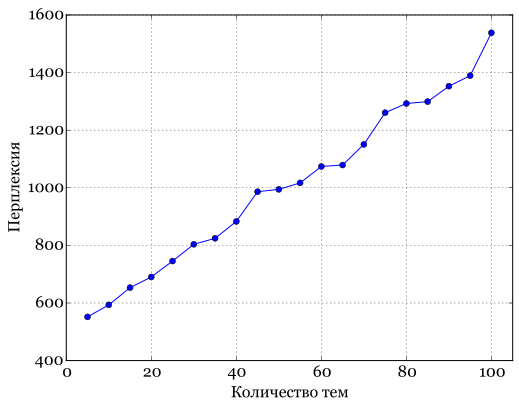
\includegraphics[totalheight=10cm]{perplexity_exp2}
    \caption{Изменение перплексии в зависимости от количества тем в программе Gensim}
    \label{fig:perplexity_gensim}
\end{figure}

Как видно из графика, в нашем случаем по мере увеличения количества тем перплексия также увеличивается, в то время как должен происходить обратный процесс -- большее количество тем лучше описывает распределение. Скорее всего это недостатки реализации расчёта перплексии в Gensim, поскольку сам автор программы признаёт наличие проблемы у некоторых пользователей\footnote{\href{https://groups.google.com/d/msg/gensim/TpuYRxhyIOc/JbTjqCcC6uYJ}{https://groups.google.com/d/msg/gensim/TpuYRxhyIOc/JbTjqCcC6uYJ}}.

Попробуем рассчитать перплексию с помощью другого инструмента и используем для этого популярную программу для тематического моделирования Mallet\footnote{\href{http://mallet.cs.umass.edu}{http://mallet.cs.umass.edu}}. Как упоминалось ранее, данная программа использует совершенно другой подход к тематическому моделированию, поэтому график \ref{fig:perplexity_mallet}, полученный в ней, сильно отличается от предыдущего. Как видно из графика, мы получили несколько локальных минимумов перплексии при 45, 60 и 85 темах.

\begin{figure}
	\centering
    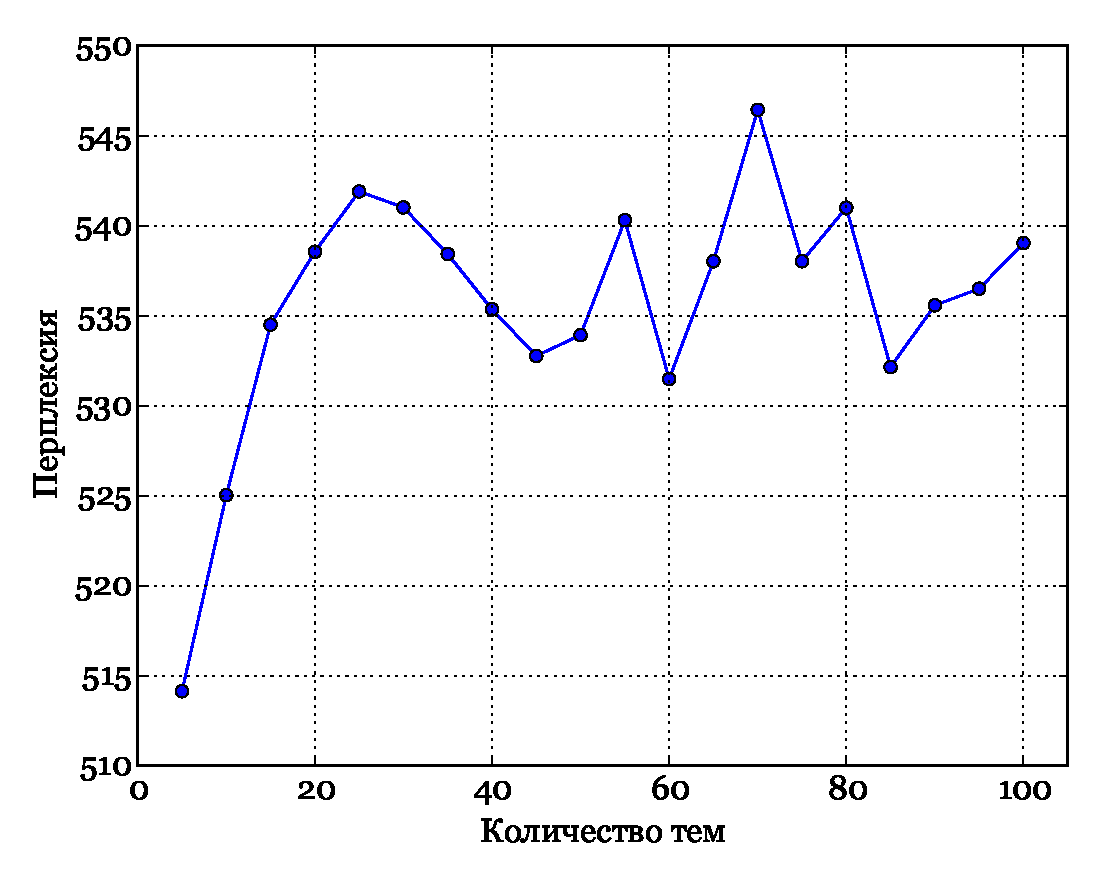
\includegraphics[totalheight=10cm]{perplexity_mallet}
    \caption{Изменение перплексии в зависимости от количества тем в программе Mallet}
    \label{fig:perplexity_mallet}
\end{figure}

Какие могут быль альтернативы расчёту перплексии? Во-первых, можно использовать алгоритмы тематического моделирования, которые автоматически подбирают оптимальное количество тем. Таким алгоритмом является, например, иерархический процесс Дирихле (hierarchical Dirichlet process, HDP), который напоминает LDA с то разницей, что данный подход относится к непараметрическим и модель сама определяет оптимальное количество тем. Так как в Gensim присутствует реализация данного алгоритма, не составит труда применить его на нашей выборке.

В результате иерархического процесса Дирихле мы получили более 500 тем. Однако данное количество тем довольно сложно интерпретировать, ведь нам необходимо проанализировать каждую тему и дать ей название.

Ещё один опробованный нами способ решения данной задачи описан в статье под названием <<О нахождении естественного числа тем в LDA: некоторые наблюдения>> \cite{Arun_KL}. В ней автор предлагает использовать расстояние Кульбака — Лейблера как способ оценки качества модели. Чем меньше указанное расстояние, тем лучше модель. В результате расчёта этого расстояния на моделях с разным количеством тем, построенных в Gensim, мы получили график, показанный на рисунке \ref{fig:kl_div}.

\begin{figure}
	\centering
    \includegraphics[totalheight=10cm]{kl_div}
    \caption{Изменение расстояния Кульбака — Лейблера в зависимости от количества тем в программе}
    \label{fig:kl_div}
\end{figure}

Из него видно, что оптимальное количество тем равняется 15, 25, 50.

В конечном итоге после сравнения моделей с разным количеством тем, мы выбрали модель с 50-ю темами, поскольку сгенерированные ей темы легче всего подвергались интерпретации и сильнее всего отличались друг от друга.

Полученные темы и их интерпретация представлены в приложении \ref{app:topics}. Как видно, в омских Интернет-СМИ представлен широкий спектр тем: от достаточно частных, касающихся ареста бывшего вице-мэра Юрия Гамбурга или убийства боксёра Ивана Климова, до взаимоотношений с Украиной и США. В случае затруднений с интерпретацией темы изучались заголовки статей, относящихся к ней с наибольшей вероятностью.

Название темы определялись после анализа слов, которые эта тема генерирует с наибольшей вероятностью. В следующем параграфе показано, как программа описывает одну из тем. Рядом с каждым словом указана вероятность, с которой оно генерируется данной темой. Из этого вероятностного распределения становится понятно, что данная тема имеет отношение к прогнозу погоды в городе Омске. Однако, как мы увидим позже, не все темы можно так легко интерпретировать.

\texttt{0.030*омск + 0.018*температура + 0.017*день + 0.015*снег + 0.014*погода + 0.014*воздух + 0.012*градус + 0.011*ветер + 0.010*область + 0.010*днём + 0.009*ожидаться + 0.009*дождь + 0.008*ночью + 0.007*выходной + 0.006*составить + 0.006*неделя + 0.006*управление + 0.006*м/с + 0.005*атмосферный + 0.005*тёплый}

Также мы можем рассчитать вероятностное тематическое распределение для каждого отдельного документа, выявив наиболее связанные с ним темы. Так как в LDA используется нечёткая кластеризация, каждый документ с некоторой вероятностью можно отнести к любой теме. %В связи с этим необходимо определить порог, который будет служить ориентиром для отнесения документа к каким-либо темам.

%Здесь мы обнаруживаем, что при пороге в 0.1 один документ в среднем можно отнести к 6.64 темам, при пороге в 0.1 -- к 2.76. При пороге в 0.2 575 документов нельзя отнести ни к одной из тем.

% Для 0.1 (2.76 среднее): 3: 11250, 2: 10010, 4: 6519, 1: 4249, 5: 1652, 6: 194, 7: 3
% Для 0.01 (6.64 среднее): 6: 4988, 5: 4596, 7: 4373, 8: 3703, 4: 3655, 9: 2906, 3: 2669, 10: 1969, 2: 1396, 11: 1232, 12: 867, 13: 489, 1: 386, 14: 275, 15: 181, 16: 90, 17: 44, 18: 32, 19: 13, 20: 8, 21: 4, 23: 1

\subsection{Тематический профиль омских Интернет-СМИ}
Итак, о чём пишут в омских Интернет-СМИ? Для ответа на этот вопрос, надо определить критерий, на основании которого среди множества выделенных ранее тем, будет выбрана та, которая будет считаться основной для данного документа или множества документов. Самый просто способ -- отнесение документа к теме, в которую он попадает с наибольшей вероятностью. Таким образом мы получим, что самая популярная тема, которая наиболее вероятная для 1855 документов -- это ДТП (тема № 19), вторая по популярности, к которой относятся 1845 документов -- преступления (тема №43), третья (1609 документов) -- взаимоотношения с Украиной (тема №39).
 
Этот способ неплохо подходит для определения темы отдельного документа, но если мы хотим таким способом оценить тематическое распределение на некотором множестве документов, то мы упустим важное преимущество LDA -- нечёткую кластеризацию, а именно возможность отнесения документа сразу к нескольким темам.

Поэтому рассмотрим другой способ решения задачи поиска наиболее популярной темы во множестве документов, решающий указанную проблему -- объединим тексты всех документов и найдём вероятностное распределение для нового большого текста. При таком подходе на первый план вышли темы 2 (сложно интерпретировать), 39 (Украина), 1 (региональная власть).

Здесь мы встречаемся с такой проблемой, как сложность интерпретации некоторых выделенных тем. В нашем случае таких тем две, а одна из них -- та самая тема номер 2 -- к тому же очень распространена. Проанализировав слова, которые она генерирует мы видим, что в них сложно найти что-то общее:

\texttt{0.009*человек + 0.007*большой + 0.006*нужно + 0.005*город + 0.005*омск + 0.005*время + 0.005*деньги + 0.005*сделать + 0.004*хороший + 0.004*вопрос + 0.004*делать + 0.004*знать + 0.004*проблема + 0.004*журналист + 0.004*работа + 0.004*работать + 0.004*должный + 0.003*проект + 0.003*метро + 0.003*думать}

К тому же вероятности, которыми тема генерирует данные слова чрезвычайно низки. Самая большая вероятность находится на уровне 0.009, в то время как в других темах примерно от 0.2 до 0.6

Одна из причин этому -- большое количество слов, которые ничего не могут сказать нам об особенностях темы. В основном это прилагательные и глаголы, которые обозначают признак предмета или его действие, но не называют сам предмет (большой, нужно, сделать, хороший и др.). Возможно, часть этих слов стоило занести в список стоп-слов.

Анализ заголовков документов, в которых проявление этой темы наиболее вероятно, также показывает сложность её интерпретации. Вот примеры заголовков некоторых из этих статей: <<Обзор блогов. Блоги – это маленькая жизнь>>, <<Сколько ещё простоят хрущевки в России?>>, <<Обзор СМИ: Страшно далеки они от народа>>, <<Кустурица стоя аплодировал омским рокерам>>. Вообще, в такие темы, как правило, попадаю статьи в жанре <<Обзор>> или <<Дайджест>>, поскольку они заключают в себе несколько тем, связанных между собой метатемой, которую при заданном уровне абстрагирования алгоритм не выделяет.

Наличие таких <<мусорных>> тем -- нормальное явление в тематическом моделировании, которого, тем не менее, надо старательно избегать, проводя качественный препроцессинг документов и выбирая оптимальное количество тем для модели. В нашем случае сложности возникли с двумя темами, что можно считать неплохим результатом. Но так или иначе, способ определения наиболее популярных тем, в котором на первое место выходит трудно интерпретируемая тема, нам не подходит

Наиболее предпочтительным нам видится третий способ определения наиболее популярных тем -- подсчёт средней вероятности для каждой темы путём сложения её вероятностей во всех документах и деления получившейся суммы на количество документов, как показано в формуле \ref{eq:popular_topics}. В этом случае мы используем все преимущества нечёткой кластеризации и получим на первых местах более содержательные темы (табл. \ref{table:popular_topics_10}).

\begin{equation}\label{eq:popular_topics}
X_b = \frac{\sum_{a=0}^{A} prob_{ab}}{A}
\end{equation}

где $A$ -- общее количество документов, $a$ -- номер документа, $b$ -- номер темы, $X_b$ -- значение популярности для темы $b$, $prob_{ab}$ -- вероятность присутствия темы $b$ в документе $a$.

В случае подсчёта по третьему методы самыми популярными у нас будут темы под номерами 19 (ДТП), 43 (преступления) и 4 (пожары). Этот способ мы считаем предпочтительным. Полные результаты представлены в таблице \ref{table:popular_topics_2} приложения \ref{app:popular_topics} на стр. \pageref{table:popular_topics_2}
\begin{longtable}[c]{| L{3cm} | C{7cm} | R{5cm} |}
	\caption{Самые популярные и не популярные темы}\label{table:popular_topics_10} 
	\\ 
	\hline
	%\multicolumn{3}{|c|}{\textbf{Файл puma\_namelist}}        \\ \hline
	\textbf{Порядок} & \textbf{Тема} & \textbf{Средняя вероятность принадлежность текстов к теме} \\ \hline
	\endfirsthead   \hline
	\multicolumn{3}{|c|}{\small\slshape (продолжение)}        \\ \hline
	\textbf{Порядок} & \textbf{Тема} & \textbf{Средняя вероятность принадлежность текстов к теме} \\ \hline
	\endhead        \hline
	\multicolumn{3}{|r|}{\small\slshape продолжение следует}  \\ \hline
	\endfoot        \hline
	\endlastfoot
		1 & 19. ДТП & 0.0478 \\
		2 & 43. Уголовные дела & 0.0448 \\
		3 & 4. Пожары & 0.0389 \\
		4 & 1. Местная власть & 0.0383 \\
		5 & 32. Бюджет Омской области & 0.0378 \\
		6 & 39. Международные отношения России, Украины и США & 0.0369 \\
		7 & 10. Суды & 0.0347 \\
		8 & 29. Хоккей: «Авангард»; «Омичка» & 0.0333 \\
		9 & 2. Сложно определить & 0.0319 \\
		10 & 7. Экономика области & 0.0313 \\
		& & \\
		... & .................................................................. & ... \\
		& & \\
		40 & 28. Концерты & 0.0106 \\
		41 & 23. Ремонт и строительство городской инфраструктуры & 0.0106 \\
		42 & 30. Хоккей: «Авангард» & 0.0103 \\
		43 & 47. Убийство Ивана Климова & 0.0097 \\
		44 & 24. Жилищный вопрос, социальная сфера & 0.0093 \\
		45 & 18. Продажа автомобилей & 0.0092 \\
		46 & 42. Торжества в честь победы в ВОВ & 0.0082 \\
		47 & 46. Таможенный контроль, правоохранительные органы & 0.0072 \\
		48 & 35. Омские СМИ: телевидение и газеты & 0.0063 \\
		49 & 27. Присоединение Крыма & 0.0062 \\
		50 & 14. Военные учения & 0.0032 \\
	\hline
\end{longtable}

Из полученных данных видно, что чаще всего исследуемые СМИ пишут на темы, связанные с насилием и бедствиями (первые три темы -- <<ДТП>>, <<Уголовные дела>>, <<Пожары>>). Пятёрку самых популярных тем замыкают две темы, касающиеся управления Омской областью (<<Местная власть>>, <<Бюджет Омской области>>).

В числе самых непопулярных тем находятся темы, касающиеся единичных событий, новости о которых актуальны ограниченный промежуток времени, пока событие себя не исчерпало: <<Убийство Ивана Климова>>, <<Торжества в честь победы в ВОВ>>, <<Присоединение Крыма>>.

\subsection{Анализ тематического профиля отдельных СМИ}\label{text:topics_by_sources}
Большие возможности для анализа открываются, если мы посмотрим, как различается тематические профили каждого из рассматриваемых СМИ. Для этого построим сводную таблицу \ref{table:popular_topics_sources}, в которой для каждой темы укажем её место в рейтинге (для наглядности перейдём от вероятностей к относительным местам) представленности рассматриваемых СМИ. Анализ этих данных позволяет узнать, насколько совпадает тематика различных СМИ и выделить издания, выбивающиеся из общего ряда, сравнить их тематический набор и сделать выводы о профиле каждого СМИ.

\begin{longtable}[c]{| C{7cm} | R{2cm} | R{2cm} | R{2cm} | R{2cm} | }
	\caption{Самые популярные темы в различных СМИ}\label{table:popular_topics_sources} 
	\\ 
	\hline
	%\multicolumn{3}{|c|}{\textbf{Файл puma\_namelist}}        \\ \hline
	\multirow{2}{*}{\bf Тема} & \multicolumn{4}{c|}{Места тем в рейтинге популярности различных СМИ}\\
		\cline{2-5}
		 & \textbf{bk55} & \textbf{ngs55} & \textbf{gorod55} & \textbf{omskinform} \\ \hline
	\endfirsthead   \hline
	\multicolumn{5}{|c|}{\small\slshape (продолжение)}        \\ \hline
	\textbf{Тема} & \textbf{bk55} & \textbf{ngs55} & \textbf{gorod55} & \textbf{omskinform} \\ \hline
	\endhead        \hline
	\multicolumn{5}{|r|}{\small\slshape продолжение следует}  \\ \hline
	\endfoot        \hline
	\endlastfoot
0. Детская медицина & 17 & 6 & 35 & 14 \\
1. Местная власть & 1 & 25 & 37 & 1 \\
2. Сложно определить & 4 & 37 & 13 & 12 \\
3. IT & 36 & 19 & 4 & 36 \\
4. Пожары & 5 & 10 & 9 & 5 \\
5. Сложно определить & 21 & 13 & 23 & 23 \\
6. Деятельность правоохранительных органов & 16 & 16 & 22 & 15 \\
7. Экономика области & 7 & 21 & 17 & 8 \\
8. Банковский сектор & 43 & 14 & 21 & 45 \\
9. Праздники, свадьбы & 22 & 24 & 18 & 44 \\
10. Суды & 10 & 8 & 24 & 4 \\
11. Организация движения и общественный транспорт & 20 & 1 & 7 & 13 \\
12. Погода & 33 & 5 & 6 & 22 \\
13. Дело Юрия Гамбурга & 32 & 47 & 29 & 39 \\
14. Военные учения & 49 & 50 & 40 & 49 \\
15. Местная власть, Горсовет & 11 & 36 & 32 & 9 \\
16. Деятельность мэрии, строительство и реконструкция & 15 & 7 & 19 & 11 \\
17. Школьные и дошкольные учреждения & 26 & 26 & 39 & 17 \\
18. Продажа автомобилей & 50 & 12 & 16 & 50 \\
19. ДТП & 6 & 2 & 2 & 3 \\
20. Высшее образование & 24 & 20 & 27 & 16 \\
21. Недвижимость: строительство, продажа & 25 & 11 & 38 & 32 \\
22. Искусство, литература & 29 & 44 & 30 & 40 \\
23. Ремонт и строительство городской инфраструктуры & 47 & 18 & 31 & 35 \\
24. Жилищный вопрос, социальная сфера & 39 & 35 & 49 & 31 \\
25. Домашние животные: собаки & 13 & 34 & 15 & 28 \\
26. Городские мероприятия & 30 & 27 & 26 & 19 \\
27. Присоединение Крыма & 45 & 49 & 44 & 47 \\
28. Концерты & 41 & 29 & 20 & 42 \\
29. Хоккей: «Авангард»; «Омичка» & 14 & 17 & 3 & 6 \\
30. Хоккей: «Авангард» & 44 & 31 & 28 & 34 \\
31. Регулирование и надзор на предприятиях & 31 & 28 & 34 & 24 \\
32. Бюджет Омской области & 8 & 3 & 10 & 7 \\
33. Объявления о поиске пропавших & 37 & 30 & 41 & 37 \\
34. Театры & 18 & 43 & 33 & 26 \\
35. Омские СМИ: телевидение и газеты & 46 & 42 & 47 & 46 \\
36. Местная власть & 9 & 48 & 43 & 18 \\
37. Экономические аспекты украинского кризиса & 23 & 40 & 14 & 41 \\
38. Коммунальная сфера: отопление & 38 & 33 & 36 & 27 \\
39. Международные отношения России, Украины и США & 3 & 45 & 1 & 29 \\
40. Информация о различных конкурсах, авиакомпании & 28 & 15 & 25 & 30 \\
41. Арбитражные суды, «Мостовик» & 12 & 22 & 46 & 21 \\
42. Торжества в честь победы в ВОВ & 40 & 39 & 45 & 38 \\
43. Уголовные дела & 2 & 4 & 11 & 2 \\
44. Фильмы, Новый год & 48 & 32 & 5 & 48 \\
45. Олимпиада 2014 & 19 & 23 & 12 & 10 \\
46. Таможенный контроль, правоохранительные органы & 42 & 41 & 42 & 43 \\
47. Убийство Ивана Климова & 35 & 38 & 50 & 33 \\
48. Сводки нарушений ПДД & 27 & 9 & 8 & 20 \\
49. Районы области & 34 & 46 & 48 & 25 \\
	\hline
\end{longtable}

Так, мы можем заметить, что сайты bk55.ru и omskinform.ru активно освещают деятельность местного самоуправления (в обоих СМИ тема <<Местная власть>> стоит на первом месте, другие родственные ей темы (15, 36) также занимают более высокое положение), в то время как у двух других новостных порталов эта тема не входит даже в первую половину рейтинга. Похожую ситуацию можно наблюдать в освещении международной политики -- только у bk55.ru и gorod55.ru данная тематика занимает передовые места в их рейтингах.

Самыми спортивно ориентированными можно назвать сайты gorod55.ru и omskinform.ru. По сравнению со своими конкурентами они уделяли больше внимания как олимпиаде в Сочи, так и выступлению региональных спортивных команд.

Достаточно интересная ситуация наблюдается с темой <<Продажа автомобилей>>. В рейтингах bk55.ru и omskinform.ru данная тема прочно занимает последнее место, в то время как в двух других оставшихся СМИ -- ngs55.ru и gorod55.ru -- входит в первую двадцатку. Можно предположить, что это следствие наличия в новостном потоке данных СМИ рекламных статей.

%Значительно более высокое место темы <<Погода>> в тематическом профиле ngs55.ru и omskinform.ru также может быть объяснено логически: в 

Ну и в заключение, мы можем дать рекомендации читателям, желающим получить максимально полную информацию, т.~е. определить два СМИ с наиболее различной тематикой -- просто посчитаем для каждой комбинации пар сумму модулей разниц их вероятностей между одинаковыми темами и выберем пару, для которой итоговое рассчитанное значение наибольшее. В итоге мы получили, что максимальная разница в темах существует между статьями с сайтов gorod55.ru и omskinform.ru, а больше всего похожи между собой bk55.ru и omskinform.ru

\begin{comment}
('bk55_preprocessed', 'gorod55')
sums 0.557354195682
('bk55_preprocessed', 'ngs55')
sums 0.567542158645
('bk55_preprocessed', 'omskinform')
sums 0.266534417882
('gorod55', 'ngs55')
sums 0.492072097932
('gorod55', 'omskinform')
sums 0.596710918679
('ngs55', 'omskinform')
sums 0.495571627246
\end{comment}

\section{Анализ комментариев}
\subsection{Введение}
В предыдущих пунктах работы мы составили тематический профиль омских Интернет-СМИ, узнав, таким образом, статьи какой тематики и в какой пропорции публикуются на сайтах исследуемых новостных ресурсов. Можно сказать, что мы исследовали их редакционные предпочтения. Следующий выделенный нами шаг -- анализ комментариев, т. е. анализ предпочтений и настроений аудитории этих СМИ. Главная цель, ради которой это затевается -- составление рейтинга тем по социальной напряжённости, индикатором которой будет служить эмоциональная тональность комментариев.

Вначале мы дадим самую общую характеристику собранным комментариям -- подсчитаем их общее и среднее количество. Затем определим самые резонансные темы, в том числе и в отдельных СМИ, проанализировав, статьи какой тематики комментирую чаще или реже всего. В заключение мы разработаем инструментарий оценки эмоциональной тональности комментариев и определим тональность комментариев к статьям различной тематики, сделав вывод об очагах социальной напряжённости.

\subsection{Общая характеристика}
Дадим общую характеристику комментариев в данном корпусе. К 26783 статьям из 33877 пользователи оставили 258121 комментариев -- в среднем этот составляет 7.6 комментария на статью.

Самая высокая комментаторская активность у аудитории сайта gorod55.ru -- 10.7 комментария на статью, самая низкая -- у omskinform.ru (2.7). Подробнее на рисунке \ref{fig:avg_comments}:
%bk55_preprocessed 8.5272094345
%ngs55 9.88509836752
%gorod55 10.6726493011
%omskinform 2.71181391085
\begin{figure}
	\centering
    \includegraphics[totalheight=10cm]{avg_comments}
    \caption{Среднее количество комментариев}
    \label{fig:avg_comments}
\end{figure}

Относительно распределения комментариев во времени, можно сказать, что оно ожидаемо практически полностью повторяет распределение статей. Подробнее на рисунке \ref{fig:comments_by_day} приложения \ref{app:comments} на стр. \pageref{fig:comments_by_day}.

\subsection{Комментируемость тем}
Определим самые резонансные темы, подсчитав, статьи какой тематики комментируют чаще всего, а какой -- реже. Для этого отнесём каждый документ к одной из тем, на основании того, к какой теме он принадлежит с наибольшей вероятностью. Затем рассчитаем отношение общего числа комментариев к статьям данной тематики к количеству этих статей. Полученное число и будет являться индикатором резонансности темы.
%[(25, 14.741982507288629), (39, 14.501243781094526), (13, 14.20414201183432), (36, 11.93984962406015), (48, 11.939705882352941), (2, 11.666666666666666), (27, 11.325714285714286), (22, 10.213058419243985), (47, 10.068592057761732), (32, 10.017227877838684), (35, 9.255172413793103), (23, 9.243027888446216), (37, 8.551063829787234), (11, 8.464699683877766), (41, 8.425096030729833), (21, 8.338530066815144), (1, 8.231625835189309), (16, 8.129562043795621), (24, 7.808035714285714), (5, 7.713768115942029), (9, 7.713603818615752), (19, 7.656418554476807), (17, 7.437858508604206), (34, 7.281399046104928), (42, 7.275862068965517), (0, 7.2066831683168315), (15, 7.127686472819216), (40, 6.427722772277228), (43, 6.4), (30, 6.347682119205298), (31, 6.001904761904762), (14, 6.0), (29, 5.90400604686319), (7, 5.847154471544715), (6, 5.493201483312732), (10, 5.476054324517513), (44, 5.266528925619835), (12, 5.248339973439575), (46, 5.246478873239437), (45, 5.137835337650324), (3, 4.810490693739425), (38, 4.743935309973046), (26, 4.7139917695473255), (4, 4.537396121883656), (33, 4.429467084639499), (20, 4.331550802139038), (49, 4.243523316062176), (28, 4.058997050147493), (8, 2.722408026755853), (18, 1.5898123324396782)]

Как и в случае с расчётом наиболее популярной темы, помня, что каждый документ можно отнести ко многим темам, мы можем внести улучшения в эту формулу. Более точные результаты можно получить, рассчитав показатель комментируемости темы путём сложения рассчитанных для каждого документа произведений вероятности присутствия темы в документе на количество комментариев в данном документе. Для того, чтобы нивелировать влияние размера темы, разделим получившееся таким образом для каждой темы значение на рассчитанный ранее показатель популярности темы. Модель расчёта показателя комментируемости представлена в формуле \ref{eq:comments_by_topics}:

\begin{equation}\label{eq:comments_by_topics}
Y_b = \frac{A \sum \limits_{a=0}^{A}prob_{ab} * qcomments_a}{\sum_{a=0}^{A} prob_{ab}}
\end{equation}
где $A$ -- общее количество документов, $B$ -- общее количество тем, $a$ -- номер документа, $b$ -- номер темы, $Y_b$ -- значение комментируемости для темы $b$, $prob_{ab}$ -- вероятность присутствия темы $b$ в документе $a$, $qcomments_a$ -- количество комментариев в документе $a$.

Полученное таким образом значение само по себе почти ничего не значит, важно лишь то, как оно различается от темы к теме. Поэтому для наглядности мы можем без последствий принять наибольшее значение комментируемости за 100\%, а для остальных тем рассчитать долю, которую они составляют от этих 100\%.

Таким образом было выявлено, что самыми комментируемыми темам являются темы, связанные с Украиной, домашними животными и арестом первого вице-мэра Омска Юрия Гамбурга. Безразличнее всего читатели отнеслись к статьям, посвящённым продаже автомобилей, банкам и чрезвычайным происшествиям (см. табл. \ref{table:comments_by_topics_10}). Полные данные представлены в таблице \ref{table:comments_by_topics} приложения \ref{app:comments} на стр. \pageref{table:comments_by_topics}.
\begin{longtable}[c]{| L{3cm} | C{7cm} | R{5cm} |}
	\caption{Более и менее всего комментируемые темы}\label{table:comments_by_topics_10} 
	\\ 
	\hline
	%\multicolumn{3}{|c|}{\textbf{Файл puma\_namelist}}        \\ \hline
	\textbf{Порядок} & \centering\textbf{Тема} & \textbf{Процент комментируемости от наиболее комментируемой} \\ \hline
	\endfirsthead   \hline
	\multicolumn{3}{|c|}{\small\slshape (продолжение)}        \\ \hline
	\textbf{Порядок} & \centering\textbf{Тема} & \textbf{Процент комментируемости от наиболее комментируемой} \\ \hline
	\endhead        \hline
	\multicolumn{3}{|r|}{\small\slshape продолжение следует}  \\ \hline
	\endfoot        \hline
	\endlastfoot
		1 & 39. Международные отношения России, Украины и США & 100.0\% \\
		2 & 25. Домашние животные: собаки & 94.0\% \\
		3 & 13. Дело Юрия Гамбурга & 86.8\% \\
		4 & 36. Местная власть & 79.9\% \\
		5 & 2. Сложно определить & 76.2\% \\
		6 & 48. Сводки нарушений ПДД & 74.9\% \\
		7 & 22. Искусство, литература & 70.3\% \\
		8 & 27. Присоединение Крыма & 69.7\% \\
		9 & 47. Убийство Ивана Климова & 67.3\% \\
		10 & 32. Бюджет Омской области & 65.7\% \\
		& & \\
		... & .................................................................. & ... \\
		& & \\
		40 & 12. Погода & 40.2\% \\
		41 & 38. Коммунальная сфера: отопление & 39.8\% \\
		42 & 44. Фильмы, Новый год & 39.6\% \\
		43 & 26. Городские мероприятия & 39.2\% \\
		44 & 45. Олимпиада 2014 & 38.7\% \\
		45 & 20. Высшее образование & 37.0\% \\
		46 & 28. Концерты & 37.0\% \\
		47 & 49. Районы области & 35.4\% \\
		48 & 4. Пожары & 34.6\% \\
		49 & 8. Банковский сектор & 34.2\% \\
		50 & 18. Продажа автомобилей & 20.7\% \\
	\hline
\end{longtable}

% [(39, 466794.4839104599), (25, 438587.41828490666), (13, 405364.2262510703), (36, 373075.0501371295), (2, 355910.23290679615), (48, 349523.98583821027), (22, 328142.3515352057), (27, 325262.4470055852), (47, 314311.9240306591), (32, 306476.511632714), (14, 303975.52692883083), (37, 303645.9904334151), (11, 288482.15107184584), (1, 287409.3612508797), (23, 284725.52456481213), (16, 274584.23424592725), (21, 273964.63247706136), (15, 270394.3898096543), (41, 268870.697295894), (42, 266407.3012991383), (35, 261548.1279847216), (19, 261130.34107368896), (9, 254836.17015757255), (5, 253670.7192758214), (24, 252749.70389157426), (0, 240659.3037026888), (17, 237992.40131337958), (34, 229088.19468558038), (43, 225123.02891694114), (46, 223780.96737727348), (40, 216745.03542798522), (31, 215439.53275631834), (7, 214176.14245982532), (6, 209028.96520340495), (10, 208889.61842837682), (30, 202085.01028213426), (3, 198766.56231538582), (29, 194878.62567135828), (33, 192648.85439201046), (12, 187617.60598127465), (38, 185746.93615677548), (44, 184636.81631191837), (26, 182812.414188796), (45, 180474.7808397816), (20, 172897.52215932752), (28, 172639.3951259277), (49, 165307.5922918495), (4, 161619.03964644053), (8, 159437.4754193113), (18, 96475.34663398893)]

В полученных данных обращает на себя внимание тот факт, что активнее всего читатели новостных порталов высказываются на тему взаимоотношений с Украиной. Соответствующие темы занимают 1, 8 и 12 места в рейтинге комментируемости. Об олимпиаде говорят хоть и не много, но, как мы увидим позже, в основном в позитивном ключе.

\subsection{Анализ тональности комментариев}
\subsubsection{Обзор методов}
Анализ тональности -- ещё одна сфера интеллектуального анализа текста. На данном этапе мы собираемся оценить эмоциональную тональность комментариев к различным темам. Гипотеза заключается в том, что если существует какая-то социальная напряжённость в обществе по отношению к какой-либо теме, то это находит выражение в комментариях к статьям соответствующей тематики. Наша задача, таким образом, состоит в том, чтобы найти темы, которые вызывают социальную напряжённость.

Существует несколько подходов к классификации тональности. Первый подход основан на наборе правил, применяя которые система делает заключение о тональности текста. Например, для предложения «Я люблю кофе», можно применить следующее правило: если сказуемое (<<люблю>>) входит в положительный набор глаголов (<<люблю>>, <<обожаю>>, <<одобряю>> ...) и в предложении не имеется отрицаний, то классифицировать тональность как <<положительная>>. Многие коммерческие системы используют данный подход, несмотря на то что он требует больших затрат, т.к. для хорошей работы системы необходимо составить большое количество правил. Зачастую правила привязаны к текстам определённой тематики (например, «ресторанная тематика») и при смене тематики («обзор фотоаппаратов») требуется заново составлять правила. Тем не менее, этот подход является наиболее точным при наличии хорошей базы правил.

Следующий подход основан на машинном обучении, чаще всего с учителем. В этом случае необходимо разметить некоторое количество текстов, на которых обучается подстроенная с помощью каких-либо алгоритмов модель. Часто для этого используется обычный байесовский классификатор. В дальнейшем эта модель распределяет тексты по заданным категориям. Недостатками метода является невысокая точность ($\approx60$\%, зависит от многих факторов) и необходимость ручной разметки обучающей выборки.

Подход, основанный на словарях, использует так называемые тональные словари (affective lexicons) для анализа текста. В простом виде тональный словарь представляет из себя список слов со значением тональности для каждого слова. Каждому слову из словаря, встречающемуся в тексте присваивается соответствующее значение, а затем вычисляется общая тональность текста. Программа, используемая в данном исследовании для оценки тональности текстов, основывается именно на этом подходе.

Вообще, по-настоящему грамотная оценка тональности, помимо определения эмоции (с помощью словаря или как-нибудь по-другому) требует ещё и определения объекта приложения этой эмоции. Например, зная о наличии негативных эмоций в комментариях к статьям на тему <<Конфликт на востоке Украины>> мы не можем сказать, к какой стороне конфликта относятся эти эмоции, что делает наше знание по большей части бесполезным. Но задача определения субъекта не имеет простого решения в рамках исследуемых методов, так что не будем затрагивать эту тему в данной работе.

\subsubsection{Выбор программы и подготовка словарей}
Существует не так много бесплатных программ, предназначенных для анализа тональности текста. Ещё меньше из них -- а в действительности ни одна из них -- умеют адекватно определять тональность текстов на русском языке. В таких сложных условиях наилучшим вариантом нам виделась программа SentiStrength\footnote{\href{http://sentistrength.wlv.ac.uk/ }{http://sentistrength.wlv.ac.uk/}} за авторством Майкла Фелвола\footnote{Глава Statistical Cybermetrics Research Group университета Вулверэмптона, ассоциированный научный сотрудник Oxford Internet Institute, Великобритания.}. Будучи бесплатной для некоммерческого использования, данная программа может работать почти с любым языком и, по крайней мере со стандартными словарями для английского языка, показывает хорошие результаты \cite{SentiStrength}. Для работы с другими языками, необходимо загрузить в неё тональные словари на нужных языках. Основания часть этих словарей представляют собой простой текстовый файл со списком слов, к каждому из которых в поставлена в соответствие оценка позитивной (по шкале от 1 до 5) или негативной составляющей (по шкале от -1 до -5). Большее значение соответствует большей выраженности эмоциональной составляющей. Другие части словаря, также представляющей собой текстовые файлы, содержат список слов-усилителей, которые усиливают значение тональности для слова, на которое они действуют (<<очень плохой>> будет иметь более негативную оценку, чем просто <<плохой>>), идиоматические выражения, слова-отрицания, смайлы, вопросительные слова, сленговые слова и слова, обозначающие иронию. Все эти части учитываются алгоритмом и помогают достичь более точного результата. Результат выдаётся в виде двух оценок – оценка позитивной составляющей текста (по шкале от +1 до +5) и оценка негативной составляющей (по шкале от -1 до -5) или в виде бинарной оценки (позитивный/негативный текст).

Но в этих же словарях кроются самые большие сложности использования программы. Первая версия словарей для русского языка\footnote{\href{http://sentistrength.wlv.ac.uk/SentStrength\_Data/russian}{http://sentistrength.wlv.ac.uk/SentStrength\_Data/russian}}, созданная факультетом прикладной лингвистики Санкт-Петербургского государственного университета аэрокосмического приборостроения, не отличается хорошим качеством. Из-за излишне общих правил данные словари часто оценивали нейтральные слова как эмоционально окрашенные\footnote{
Дело в том, что в словарях к SentiStrength для создания простых правил можно использовать оператор *, который обозначает любое количество любых символов кроме пробела. Под шаблон <<*плом*>>, например, подходят слова <<\textbf{плом}ба>>, <<ди\textbf{плом}ированный>> и др. В своих словарях авторы переусердствовали с применением данного оператора. Это привело, например, к тому, что словари дают три балла негативной эмоциональной составляющей любому слову, начинающемуся на <<ад>> (приравнивая \textbf{ад}министраторов к исчадиям \textbf{ад}а) и два балла позитивной словам на <<мил>> (а это далеко не только слово <<\textbf{мил}ый>>, как вероятно задумывали авторы словарей, но и вызывающее не самые позитивные эмоции слово <<\textbf{мил}иция>>).
}.

\begin{comment}
Особенности SentiStrength:
Чтобы слова-отрицатели на русском работали без проблем, надо поставить перед ними английское слово

Слова с модулем тональности 1 не влияют на оценку (возможно они нужны, чтобы давать баллы, находясь рядом со словами-усилителями)
\end{comment}

Вероятно, по этой причине для своего исследования тональности комментариев к постам в Живом Журнале коллективом Лаборатории Интернет-Исследований был создан новый тональный словарь\footnote{\href{http://sentistrength.wlv.ac.uk/SentStrength\_Data/russian2}{http://sentistrength.wlv.ac.uk/SentStrength\_Data/russian2}}\cite{hse_sentistrength}. Процесс адаптации включал в себя перевод англоязычного словаря, на основе которого работает ПО, на русский язык, подбор подходящих русских эквивалентов полученным словам, составление частотного словаря на основе комментариев к постам ЖЖ, включение частотных слов в словарь и кодирование словаря по шкале эмоциональности от -5 до 5. После сопоставления результатов работы программы с результатами ручного кодирования был сделан вывод, что количество совпадений между автоматическим кодированием с данным словарём и ручным кодированием с помощью экспертов значительно уступает результатам аналогичных экспериментов на английском языке.

По сравнению с первым вариантом словаря, второй вариант обладал прямо противоположной проблемой -- тенденцией оценивать негативно эмоционально окрашенные тексты как нейтральные\footnotemark \cite[стр. 3]{hse_sentistrength}. 

\footnotetext{
	Нами было выделено несколько вероятных причин проблем у второго варианта словаря. Главная из них заключается в том, что словарь состоит только из слов в нормальной форме и оператор * в них не используется. Поэтому для оценки текстов с использованием этого словаря необходима предварительная лемматизация. Сотрудники Лаборатории Интернет-исследований, естественно, знали об особенностях своих словарей и не обошли вниманием этот этап.
	
	Здесь, однако, стоит сказать, что лемматизация достаточно плохо работает на словах, которые ярче всего свидетельствуют о негативных эмоциях -- обсценной лексике. Для лемматизации необходим словарь со всеми словоформами, но мат в эти словари включают редко.
	
	К тому же, многие программы, производящие лемматизацию (тот же используемый нами pymorphy2), при приведении слова к нормальной форме не отбрасывают при этом приставки (<<набрал>> $\rightarrow$ <<набрать>>, а не <<брать>>), которые играют огромную роль в обсценной лексике. В такой ситуации необходимо включать в словарь слова обсценной лексики со всеми вариантами приставок, что сложно при наличии проблемы, указанной в предыдущем абзаце.

	Ещё одна возможна причина неудовлетворительного результата работы второго варианта словаря может заключаться в том, что для перед лемматизацией необходима токенизация. Но SentiStrength предназначена для анализа <<сырого>> текста сама производит токенизацию по своему специфическому алгоритму. Так конструкция <<какое-либо-слово)))>> благодаря тому, что смайл и слово являются одним целым, будет присвоено два балла положительного эмоционального заряда. Но если отделить смайл от слова <<какое-либо-слово )))>>, то программа просто не увидит здесь никакой эмоции.

	Возможно, лучший результат дала бы замена лемматизации на стемминг. Так как для стемминга не нужна база основ слов, а лишь правила и набор морфем, проблема обсценных слов была бы решена.
}

%На сайте SentiStrength был найден ещё один словарь, происхождение которого нам неизвестно \footnote{\href{http://sentistrength.wlv.ac.uk/SentStrength\_Data/russian/Russian\%20May\%202011.zip}{http://sentistrength.wlv.ac.uk/SentStrength\_Data/russian/Russian May 2011.zip}}. В нём не использовался оператор *, но словарная база превосходила по объёму второй вариант словаря. Впрочем, не все слова из этого словаря были адекватно оценены (аргумент -2, аккумуляторов -2). Вероятно, данный словарь создавался для оценки текстов специфической тематики, и там такая оценка тональности была корректна, но в нашем случае лучше будет избавиться от неё.

Также общим недостатком рассматриваемых русскоязычных словарей является практически полное отсутствие в них идиоматических выражений, сленговых и ироничных слов.

В условиях невысокого качества словарей, было принято решение о создании нового тонального словаря. В целях экономии ресурсов было решено построить его на основе предыдущих версий, учтя их достоинства и недостатки, с добавлением специфичных для исследуемых текстов эмоционально окрашенных слов.

Моделью для построения нового словаря стал первый словарь, основанный на правилах. Из него были удалены правила, касающиеся слов меньше, чем из четырёх символов и допускающие некорректные соответствия словам (правило ад* допускало соответствие слову администратор). Затем правила были преобразованы в обычные слова (ад). Далее все слова (только слова, не правила) с помощью программы pymorphy2, были развёрнуты в свои всевозможные словоформы (ад, ада, адом и др.) Таким образом явное указание подходящих слов позволило уйти от слишком общих правил.

Второй словарь, который, напомним, состоял только из нормальных форм и требовал лемматизации поступающих текстов, было решено преобразовать к формату первого. Для этого длинные слова данного словаря были пропущены через процедуру стемминга с последующей заменой усечённых частей на оператор *. Для более коротких слов, как и в предыдущем случае, были найдены все словоформы.

Затем получившиеся словари были объединены и к ним добавили 113 тональных слов, выделенных на основании изучения более двухсот случайных комментариев из исследуемой выборки и отсутствующих в исходных словарях. Некоторые их этих слов специфичны для текстов, написанных в исследуемый промежуток времени (например, слово <<укроп>>). Баллы данным словам присваивались на основе анализа контекста и мнения автора об их эмоциональной тональности. Эта стратегия не идеальна, поскольку выставляемые оценки отражают субъективное мнение одного человека. В дальнейших исследованиях при наличии ресурсов для оценки эмоциональной тональности следует привлекать нескольких экспертов и, затем, проверять надёжность интеркодирования с последующей корректировкой оценок в случае значительных расхождений.

Конструирование нового словаря закончилось удалением повторяющихся записей.

Новый словарь обладает следующими преимуществами:

\begin{enumerate}
\item Он объединяет словарные базы двух разных словарей -- а значит полнее каждого из них по отдельности.
\item В отличие от второго словаря, для пользования данным словарём не надо модифицировать входящие данные.
\item Правила нового словаря корректнее, точнее, чем правила первого словаря, что означает меньшее количество ложных оценок.
\item Данный словарь включает слова, которых не было ни в одном из предыдущих.
\end{enumerate}

Далее необходимо оценить эффективность определения тональности с использованием нового словаря по сравнению с предшественниками. Для этого была использована коллекция цитат из новостного потока с разметкой по оценочной тональности, предоставленная РОМИП\footnote{Российский семинар по оценке методов информационного поиска (РОМИП) — это открытый семинар, проводимый ежегодно с 2003 года группой российских исследователей и разработчиков, занимающихся информационным поиском. Основная цель семинара — создание плацдарма для проведения независимой оценки методов информационного поиска, ориентированных на работу с русскоязычной информацией. Структурно семинар представляет собой набор дорожек — секций, посвящённых конкретным проектам с определенной задачей и правилами оценки. Оргкомитет формирует тестовые наборы данных, заданий и распространяет их участникам. Участник самостоятельно и на своём оборудовании выполняет поисковые задания интересующих его дорожек, и затем предоставляет результаты (ответы) оргкомитету в оговорённые сроки. Одним из видов заданий, выполняемых участниками, является определение тональности текстов.

Для данного исследования по запросу автора РОМИП предоставил одну из своих тестовых коллекций: \url{http://romip.ru/ru/collections/sentiment-news-collection-2012.html}}. Данная коллекция состоит из 4260 оценок. Оценка может принимать одно из 4-х значений: положительная, отрицательная, смешанная и нет оценки. Для простоты тестирования тексты со смешанными оценками были исключены.

Вариант словаря созданный факультетом прикладной лингвистики на тестовой коллекции показал точность оценивания в 47\%. Использование созданного нами словаря позволило увеличить точность оценивания до 50\%. Много это или мало?

Для начала следует сказать, что тестовую выборку составляли отрывки из новостных статей. Сравнивая эти рафинированные тексты, написанные профессиональными журналистами, с реальными комментариями, следует заметить, что эмоциональная тональность последних, как правило, выражена гораздо чётче. Это замечание позволяет предположить, что в приложении к реальным комментариям эффективность оценивания несколько повысится.

Далее отметим, что по результатам тестов, проведённых автором программы, на англоязычных текстах с использованием соответствующих словарей SentiStrength показывается точность в 60\% (что лучше, чем большинство других программ) \cite{SentiStrength}. Исследователям из ВШЭ удалось добиться точности работы на русскоязычных текстах от 40\% до 48\% \cite[стр. 49]{kolcova_sentistrength}.

Исходя из сказанного, нельзя считать полученный нами результат в 50\%, особенно с учётом характера тестовой коллекции, абсолютно провальным. Необходимо понимать, что даже для английского языка точность определения тональности выше 70\% считается практически идеальной. Однако и хорошим признать полученный результат тоже нельзя. Алгоритмы, основанные на машинном обучении, по оценке того же Майкла Фелвола, позволяют добиться точности до 58,5\%. И это при том, что эффективность данных методов почти не зависит от языка. Их минусами, как уже говорилось ранее, является необходимость в большой обучающей выборке и более высокая сложность использования.

\subsubsection{Определение тональности по темам}
Настало время задействовать полученные словари и посмотреть различия в настроениях комментирующих от темы к теме. Формула расчёта общей тональности темы \ref{eq:senti_topics} похожа на формулу комментируемости \ref{eq:comments_by_topics} (стр. \pageref{eq:comments_by_topics}) с той лишь разницей, что количество комментариев заменено на среднюю оценку эмоциональной тональности комментариев в данном документе.

\begin{equation}\label{eq:senti_topics}
Z_b = \frac{A \sum \limits_{a=0}^{A}prob_{ab} * avgSenti_a}{\sum_{a=0}^{A} prob_{ab}}
\end{equation}
где $A$ -- общее количество документов, $B$ -- общее количество тем, $a$ -- номер документа, $b$ -- номер темы, $Z_b$ -- значение тональности для темы $b$, $prob_{ab}$ -- вероятность присутствия темы $b$ в документе $a$, $avgSenti_a$ -- средняя оценка тональности комментариев в документе $a$.

Как и раньше, полученные таким образом числа обретают смысл только в сравнении друг с другом, поэтому примем значение тональности максимально позитивной темы за 100\%, а для остальных тем рассчитаем значения относительно этих процентов.

Результаты анализа вполне логичны, но от этого не менее интересны. Крайние темы этого рейтинга представлены в таблице \ref{table:senti_topics_10}. Наибольшие позитивные эмоции у комментаторов вызвало, наверное, главное событие 2014 года в России -- олимпиада в Сочи. Вслед за ней своё место в сердцах читателей нашли темы, касающиеся информации о конкурсах, театрах, праздниках и свадьбах, концертах, городских мероприятиях и известных спортивных клубах. Негативные эмоции, а, следовательно и социальную напряжённость, вызвали такие темы как <<Уголовные дела>>, <<Убийство Ивана Климова>>, <<ДТП>> и, довольно неожиданно, <<Детская медицина>>, опередившая даже следующие за ней темы <<Пожары>> и <<Сводки нарушений ПДД>>. Полные данные можно найти в таблице \ref{table:senti_topics} приложения \ref{app:comments} на стр. \pageref{table:senti_topics}.
%[(45, 10851.396275175188), (40, 10177.501709043183), (34, 10165.379971862409), (9, 8366.502517378613), (28, 8192.27805789244), (26, 7473.353622137029), (29, 6418.366255023755), (21, 5704.325366789691), (1, 5593.068046355217), (27, 5183.203889597853), (12, 5150.721527266371), (20, 5112.203425555053), (30, 5103.323102791469), (42, 4977.66825359893), (2, 4903.501546732583), (7, 4540.605718165502), (18, 4404.720520481995), (44, 4142.947771631055), (35, 4121.452850488652), (16, 3933.597936675806), (5, 3906.869560255782), (17, 3487.1259454620213), (8, 3385.206713884894), (23, 3384.310355932247), (32, 3151.2699841600806), (11, 3123.0721289164694), (22, 2827.7424934322785), (3, 2568.399600558708), (36, 2516.8177041975305), (15, 2371.580916824568), (38, 2208.554125326193), (24, 1882.4722417498056), (41, 1475.8702470996934), (37, 957.7712432405326), (49, 910.3404522529037), (14, -181.62945908732397), (13, -316.6242322253222), (25, -356.6190716989229), (33, -1501.655616845577), (46, -1521.988932354942), (10, -1878.457295670864), (39, -2101.0230010187584), (31, -2376.5865450847637), (6, -3676.779010760171), (48, -4821.610281369253), (4, -5466.785720006037), (0, -5628.21553684776), (19, -8749.692475178386), (47, -10593.013148092621), (43, -11121.020128372396)]

Содержательная интерпретация получившихся результатов требует обратить внимание на две выделяющиеся из общего ряда темы. Первая из них -- <<Убийство Ивана Климова>>. Данная тема относится к одному событию, в то время как остальные темы, вызывающие негативные эмоции, затрагивают не события, а, скорее, явления или институты. Присутствие локальной темы в списке смоделированных алгоритмом тем, да ещё с такими высокими показателями комментируемости и негативной эмоциональной тональности комментариев к ней, свидетельствует об очень большой социальной напряжённости в данном вопросе.

Следует обратить внимание и на другое исключение -- присутствие темы <<Детская медицина>> на четвёртом месте в рейтинге тем, вызывающих у читателей наиболее сильные негативные эмоции. В отличии от остальных тем, находящихся на первых местах этого рейтинга, данная тема сама по себе не должна вызывать сильных негативных эмоций. Текущая же ситуация свидетельствует о явном недовольстве омичей системой детского здравоохранения.
\begin{longtable}[c]{| L{3cm} | C{7cm} | R{5cm} |}
	\caption{Темы с самыми положительными и отрицательными комментариями}\label{table:senti_topics_10} 
	\\ 
	\hline
	%\multicolumn{3}{|c|}{\textbf{Файл puma\_namelist}}        \\ \hline
	\textbf{Порядок} & \textbf{Тема} & \textbf{Процент от наиболее позитивной} \\ \hline
	\endfirsthead   \hline
	\multicolumn{3}{|c|}{\small\slshape (продолжение)}        \\ \hline
	\textbf{Порядок} & \textbf{Тема} & \textbf{Процент от наиболее позитивной} \\ \hline
	\endhead        \hline
	\multicolumn{3}{|r|}{\small\slshape продолжение следует}  \\ \hline
	\endfoot        \hline
	\endlastfoot
		1 & 45. Олимпиада 2014 & 100.0\% \\
		2 & 40. Информация о различных конкурсах, авиакомпании & 93.8\% \\
		3 & 34. Театры & 93.7\% \\
		4 & 9. Праздники, свадьбы & 77.1\% \\
		5 & 28. Концерты & 75.5\% \\
		6 & 26. Городские мероприятия & 68.9\% \\
		7 & 29. Хоккей: «Авангард»; «Омичка» & 59.1\% \\
		8 & 21. Недвижимость: строительство, продажа & 52.6\% \\
		9 & 1. Местная власть & 51.5\% \\
		10 & 27. Присоединение Крыма & 47.8\% \\
		& & \\
		... & .................................................................. & ... \\
		& & \\
		40 & 46. Таможенный контроль, правоохранительные органы & -14.0\% \\
		41 & 10. Суды & -17.3\% \\
		42 & 39. Международные отношения России, Украины и США & -19.4\% \\
		43 & 31. Регулирование и надзор на предприятиях & -21.9\% \\
		44 & 6. Деятельность правоохранительных органов & -33.9\% \\
		45 & 48. Сводки нарушений ПДД & -44.4\% \\
		46 & 4. Пожары & -50.4\% \\
		47 & 0. Детская медицина & -51.9\% \\
		48 & 19. ДТП & -80.6\% \\
		49 & 47. Убийство Ивана Климова & -97.6\% \\
		50 & 43. Уголовные дела & -102.5\% \\
	\hline
\end{longtable}
Если говорить о темах с наиболее позитивными комментариями, то их высокие места в этом рейтинге вполне логичны, поскольку все из них касаются событий, предназначенных для поднятия настроения -- праздников, концертов, спортивных мероприятий и т. д (темы 1-7). Первыми темами, на верхушке рейтинга, выбивающимися это этого ряда, являются темы <<Недвижимость: строительство и продажа>> и <<Местная власть>>, расположенные на 8 и 9 местах.

Также интересно, что читатели в позитивных тонах комментировали присоединение Крыма и в негативных -- взаимоотношения с Украиной. Такое интуитивно соответствующее реальной ситуации различие свидетельствует о том, что модели удалось разграничить эти тесно связанные темы.

\subsubsection{Определение тональности по темам в различных СМИ}
Для исследователя-маркетолога может быть полезно рассмотреть различия в отношении к выделенным темам комментирующей аудитории каждого из выделенных СМИ в отдельности. Для этого мы составим матрицу рейтинга положительного отношения к темам в каждом СМИ. Под рейтингом положительного отношения имеется ввиду место, которое каждое тема занимает в списке тем, отсортированных от положительного отношения к отрицательному. Ранее мы сделали выводы о тематическом предпочтении редакторов СМИ (пункт \ref{text:topics_by_sources}). Анализ новых данных позволяет делать предположения о предпочтениях их аудитории.

Вряд ли можно рассчитывать, что эмоциональная оценка авторов комментариев к статьям рассматриваемых СМИ будет сильно отличаться, поскольку все эти сайты рассчитаны на одну и ту же аудиторию и предоставляют сходный контент. Более интересно было бы проанализировать различие эмоционального отношения к одним и тем же темам приверженцев СМИ, представляющих полярные политические или даже мировоззренческие позиции. Но в таком случае мы могли бы столкнуться с проблемой малого количества общих тем в их тематическом наборе. Так или иначе, взглянем на наши данные в таблице \ref{table:senti_topics_sources}, приложение \ref{app:comments}, стр. \pageref{table:senti_topics_sources}.

Посмотрев на места тем 29 (Хоккей: «Авангард»; «Омичка») и 30 (Хоккей: «Авангард») мы можем сказать, что по сравнению с аудиторией других сайтов, аудитория сайта gorod55.ru испытывает более негативные эмоции относительно спортивных успехов омских команд. Зато они позитивнее отзываются о городских мероприятиях (тема 26) и деятельности мэрии в общем (темы 16, 10). Комментирующие с сайта omskinform.ru более других позитивны в отношении других омских СМИ (тема 35), но почему-то скептически настроены к новостям о погоде (тема 12).


\clearpage